
We know that the total probability is one,
\begin{equation}
    \int_{-\infty}^{\infty}{f\brak{x} dx} = 1\label{b}
\end{equation}
Using \eqref{a} in \eqref{b},
\begin{align}
    \int_{0}^{1}{(a+bx)\,dx} = 1\\
    \sbrak{ax+\frac{bx^2}{2}}_0^1=1\\
    \left(a+\frac{b}{2}\right)-0=1\\
    \implies a+\frac{b}{2}=1 \label{c}
\end{align}
We know that expectation value of X,
\begin{align}
    E\brak{X}=\int_{-\infty}^{\infty}xf\brak{x}\,dx\label{d}
\end{align}
%
Using $E\brak{X}=\frac{2}{3}$ and \eqref{a} in \eqref{d}, we get
\begin{align}
     \frac{2}{3}&=\int_{0}^{1}x(a+bx)\,dx\\
     &=\int_{0}^{1} ax+bx^2\,dx\\
     &= \sbrak{\frac{ax^2}{2}+\frac{bx^3}{3}}_0^1\\
     &= \frac{a}{2}+\frac{b}{3}-0\\
     \implies\frac{a}{2}+\frac{b}{3}&=\frac{2}{3}\label{e}
\end{align}
By solving \eqref{c} and \eqref{e}, we get 
\begin{align}
    a\, =\, 0 \,\,and\,\, b\, =\, 2.
\end{align}
Using values of $a$ and $b$ in \eqref{a}, we get
\begin{align}
f\brak{x}
= 
\begin{cases}
2x & 0<x<1
\\
0 & otherwise\label{f}\\
\end{cases}
\end{align}
\begin{figure}[ht]
    \centering
    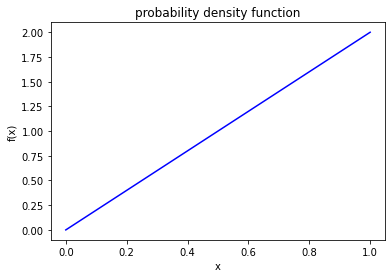
\includegraphics[width=\columnwidth]{solutions/ec/15/figures/assign2.png}
    \caption{Probability Density Function (PDF) of X}
    \label{Figure_1}
\end{figure}
The graph of PDF of X is \ref{Figure_1}
\par Let $F_X(x)$ be the cumulative distribution function of random variable X.
\begin{align}
    F_X(x)=\int_{-\infty}^x f\brak{x} dx\label{x}
\end{align}
$F_X(x)$ can be obtained from the uniform distribution of a random variable U on (0,1) and let U=$X^2$. 
\begin{align}
    0 < U < 1
\end{align}
As for random variable X also,
\begin{align}
    0 < F_X(x) < 1
\end{align}
This similarity between U and $F_X(x)$ is used to generate the random variable X from U.
\begin{align}
    F_X(x)&= \pr{X<x}\\
    &=\pr{\sqrt{U}<x}\\
    &=\pr{U<x^2}\\
    &=F_U(x^2)\label{y}
\end{align}
From uniform distribution,
\\The graph of Probability Density Function (PDF) of U is \ref{Figure_2}
\begin{figure}[ht]
    \centering
    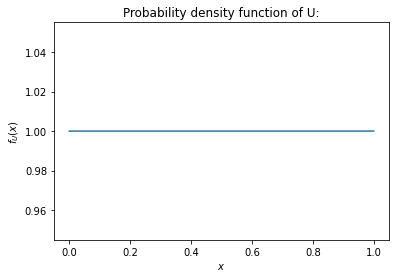
\includegraphics[width=\columnwidth]{solutions/ec/15/figures/assign2_2.png}
    \caption{Probability Density Function (PDF) of U}
    \label{Figure_2}
\end{figure}
\begin{align}
    F_U(x)=
    \begin{cases}
0 & x\leq0\\
x & 0<x<1
\\
1 & x\geq1\label{z}\\
\end{cases}
\end{align}
\begin{figure}[ht]
    \centering
    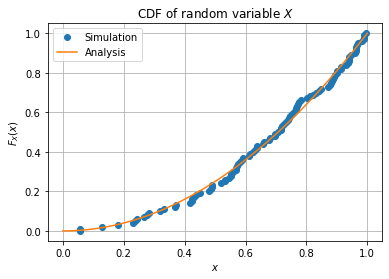
\includegraphics[width=\columnwidth]{solutions/ec/15/figures/assign2_1.png}
    \caption{Cumulative Density Function (CDF)}
    \label{Figure_3}
\end{figure}
\\Using \eqref{z} in \eqref{y},
\\Cumulative distribution function (CDF) of random variable X is,
\begin{align}
F_X(x)= \pr{X<x}
= 
\begin{cases}
0 & x\leq0\\
x^2 & 0<x<1
\\
1 & x\geq1\label{g}\\
\end{cases}
\end{align}
The graph of Cumulative distribution function (CDF) of random variable X is \ref{Figure_3}\\
Now we have to find \pr{X<0.5},Using  \eqref{g},
\begin{align}
    \pr{X<0.5} &= (0.5)^2\\
  \implies \pr{X<0.5} &= 0.25
\end{align}

